\documentclass[conference]{IEEEtran}
\IEEEoverridecommandlockouts
% The preceding line is only needed to identify funding in the first footnote. If that is unneeded, please comment it out.
\usepackage{cite}
\usepackage{amsmath,amssymb,amsfonts}
\usepackage{algorithmic}
\usepackage{graphicx}
\usepackage{textcomp}
\usepackage{xcolor}
\usepackage{url}
\usepackage{hyperref}
\usepackage{float}
\usepackage{moresize}

\makeatletter
\newcommand{\linebreakand}{%
  \end{@IEEEauthorhalign}
  \hfill\mbox{}\par
  \mbox{}\hfill\begin{@IEEEauthorhalign}
}
\makeatother



\def\BibTeX{{\rm B\kern-.05em{\sc i\kern-.025em b}\kern-.08em
    T\kern-.1667em\lower.7ex\hbox{E}\kern-.125emX}}
\begin{document}

\title{¿Quién gasta más y quién se registra? Evidencia observacional en CheMarket}

\author{%
\IEEEauthorblockN{Adrián Arturo Suárez García}
\IEEEauthorblockA{202123771\\
\href{mailto:a.suarezg@uniandes.edu.co}{\texttt{a.suarezg@uniandes.edu.co}}}
\and
\IEEEauthorblockN{Luis Alejandro Rubiano Guerrero}
\IEEEauthorblockA{202013482\\
\href{mailto:la.rubiano@uniandes.edu.co}{\texttt{la.rubiano@uniandes.edu.co}}}
\and
\IEEEauthorblockN{Gabriel Alejandro Moreno Riveros}
\IEEEauthorblockA{202014583\\
\href{mailto:g.morenor@uniandes.edu.co}{\texttt{g.morenor@uniandes.edu.co}}}
\linebreakand
\IEEEauthorblockN{Juan Sebastián Sierra Tarazona}
\IEEEauthorblockA{202123725\\
\href{mailto:j.sierrat@uniandes.edu.co}{\texttt{j.sierrat@uniandes.edu.co}}}
}



\maketitle


\section{Introducción}
A través de este informe, nuestro grupo de economistas y científicos de datos emplea diferentes técnicas de análisis estadístico y de machine learning para estudiar el comportamiento de los usuarios en \textbf{CheMarket Inc.} En particular, nos enfocamos en entender qué variables impulsan el revenue de la compañía, con el fin de generar evidencia que apoye la toma de decisiones estratégicas informadas.

El análisis se divide en dos partes complementarias. En la primera parte, trabajamos con datos observacionales para explorar patrones en el comportamiento de los usuarios: ¿quiénes gastan más?, ¿qué factores están asociados con el registro en la plataforma?, ¿qué variables ayudan a predecir el gasto individual? A partir de regresiones y modelos predictivos evaluamos si existe una diferencia sistemática en el gasto entre usuarios registrados y no registrados, y discutimos posibles sesgos que afectan la interpretación causal.

En la segunda parte, analizamos un experimento aleatorio en el que se facilitó el proceso de registro para un grupo de usuarios. Esta intervención nos permite estimar de manera más rigurosa el efecto del registro sobre el gasto, así como evaluar la efectividad del nuevo diseño en incrementar la tasa de registros. Finalmente, reflexionamos sobre la validez de los resultados, las limitaciones del experimento y presentamos recomendaciones concretas sobre si conviene escalar esta intervención.

\section{Datos observacionales: ¿Qué impulsa las ventas?}

\subsection{Datos y preparación}

Para el análisis observacional, contamos con un conjunto de $100.000$ observaciones históricas de los usuarios de CheMarket. Las variables disponibles son $\texttt{time\_spent}$: tiempo en el sitio durante la sesión, $\texttt{past\_sessions}$: número de sesiones anteriores, 
$\texttt{device\_type}$: tipo de dispositivo (móvil, escritorio, tablet), $\texttt{os\_type}$: sistema operativo (OS X, Windows, otros), $\texttt{is\_returning\_user}$: si el usuario ya había visitado antes, $\texttt{sign\_up}$: si se registró o no y $\texttt{revenue}$: cuanto gastó en cada sesión.

En la siguiente tabla se presentan las estadísticas descriptivas de estas variables.


\begin{table}[H]
\ssmall
\centering
\caption{Estadísticas descriptivas de las variables}
\begin{tabular}{|l|c|c|c|c|c|c|}
\hline
 & \textbf{Tiempo} & \textbf{Sesiones} & \textbf{Dispositivo} & \textbf{OS} & \textbf{Recurrente?} & \textbf{Revenue} \\
\hline
Mín & 0.000125 & 0 & Tablet: 9882 & Otro: 9909 & No: 4930 & 0.5451 \\
25\% & 1.4247 & 2 & Escritorio: 40009 & OS X: 30253 & Sí: 95070 & 2.3400 \\
Mediana & 3.4384 & 3 & Móvil: 50109 & Windows: 59838 & & 3.1370 \\
50\% & 4.9946 & 3.001 & & & & 3.9766 \\
75\%  & 6.9117 & 4  & & & & 4.5221 \\
Máx & 54.3989 & 14  & & & & 36.2934 \\
\hline
\end{tabular}

\hfill \break
Estadísticas descriptivas de las variables numéricas y cantidad por clase para las categóricas.

\end{table}

En la siguiente figura se presentan las distribuciones originales de \texttt{Revenue} y \texttt{time\_spent}.
Se puede observar que la densidad de ambas variables muestra muchos valores pequeños y pocos muy grandes.
Para nuestro análisis decidimos aplicar una transformación logarítmica y de raíz cuadrada respectivamente,
ya que estas transformaciones comprimen la cola y acercan la distribución a algo más gaussiano, 
lo que beneficia métodos lineales y tests que asumen normalidad de errores.


\begin{figure}[H]
    \centering
    \includegraphics[width=0.3\textwidth]{figures/revenueA.png}

    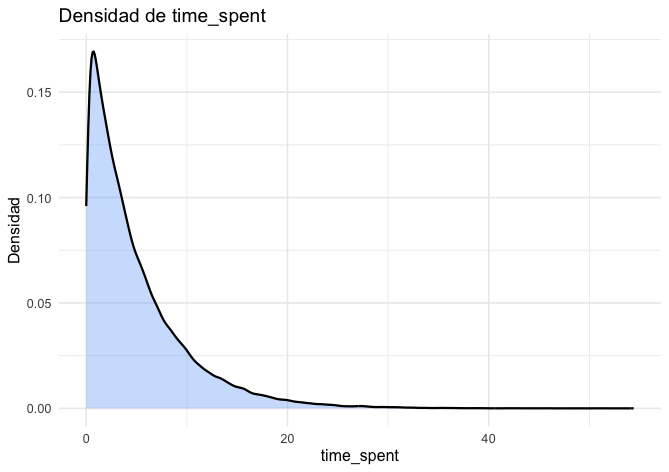
\includegraphics[width=0.3\textwidth]{figures/timespentA.png}
    \caption{Distribución de \texttt{Revenue} y \texttt{time\_spent}}
    \label{fig:distribucion}
\end{figure}


Partición


\subsection{Estimación del efecto de registrarse}

Marco conceptual, sesgo por variables omitidas.


Densidades

Histogramas

Boxplot

\subsection{Efecto de registrarse sobre el gasto}


Diferentes modelos

pseudo coefplot coeficientes

Interpretación

multicolinealidad


\subsection{Reflexión sobre causalidad y recomendación preliminar}


\section{Datos experimentales: ¿Funciona facilitar el registro?}

\subsection{Verificación del experimento}

\subsection{Efecto sobre el registro}

\subsection{Efecto sobre el gasto}

\subsection{Limitaciones y robustez}

\subsection{Recomendación final}

\section{Conclusiones}

Resumen 

Recomendaciones accionables.



\end{document}
